\textbf{COLUNI 2020 -- Questão 28}\par\medskip O mosquito \textit{Aedes aegypti} é originário da África subsaariana (aedes = odioso; aegypti = do Egito) e se dispersou com grande facilidade para todos os continentes por diferentes meios de transporte. Há relatos de que o mosquito chegou ao Brasil pela primeira vez em navios que faziam o transporte de escravos durante a colonização portuguesa. O ciclo de vida do mosquito inicia-se quando os ovos eclodem, as larvas transformam-se em pupas e os adultos emergem, como ilustrado a seguir:

% COLUNI-AUTO-FIGURES-BEGIN
\begin{figure}[htbp]
\centering
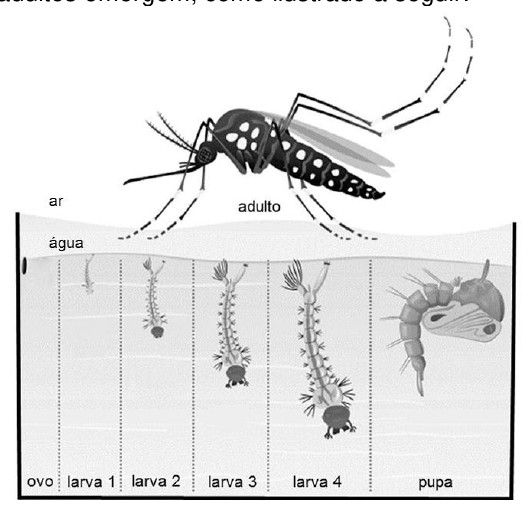
\includegraphics[width=0.95\linewidth]{static/simulados/coluni/figuras/2020/questao-28/figura-1.png}
\end{figure}
% COLUNI-AUTO-FIGURES-END

\par

Fonte: https://educador.brasilescola.uol.com.br/estrategias-ensino/verificando-existencia-aedes-aegypti.htm. Acesso em: 19 ago 2019. (Adaptado)

\par

Sobre o \textit{Aedes aegypti}, analise as afirmativas a seguir:

\par

I.     Os ovos resistem ao ressecamento, e as larvas nascem quando os ovos são reidratados. \\
II.    Os imaturos habitam lagos e riachos, e os adultos, o interior de residências e florestas. \\\
III.   As larvas alimentam-se de microrganismos e detritos em decomposição, e as fêmeas adultas, de sangue. \\\
IV.    As larvas respiram por brânquias externas, e as pupas, por trocas através da superfície do corpo. \\\
V.     Os imaturos podem ser eliminados por inseticidas em água, e os adultos, por pulverização de inseticida por fumacê.

\par

Está CORRETO o que se afirma apenas em:

\begin{enumerate}
\item I, II e IV.
\item II, III e IV.
\item I, III e V.
\item III, IV e V.\end{enumerate}
